The model achieve a training accuracy of 99.29\% and a validation accuracy of 99.31\%. \autoref{f:accuracy_plot} 
and \autoref{f:loss_plot} display the performance of the model during training. A confusion matrix analysis 
revealed that the model performed well across all digit classes, with most misclassifications occurring between 
visually similar digits. 

\begin{figure}
  \begin{center}
    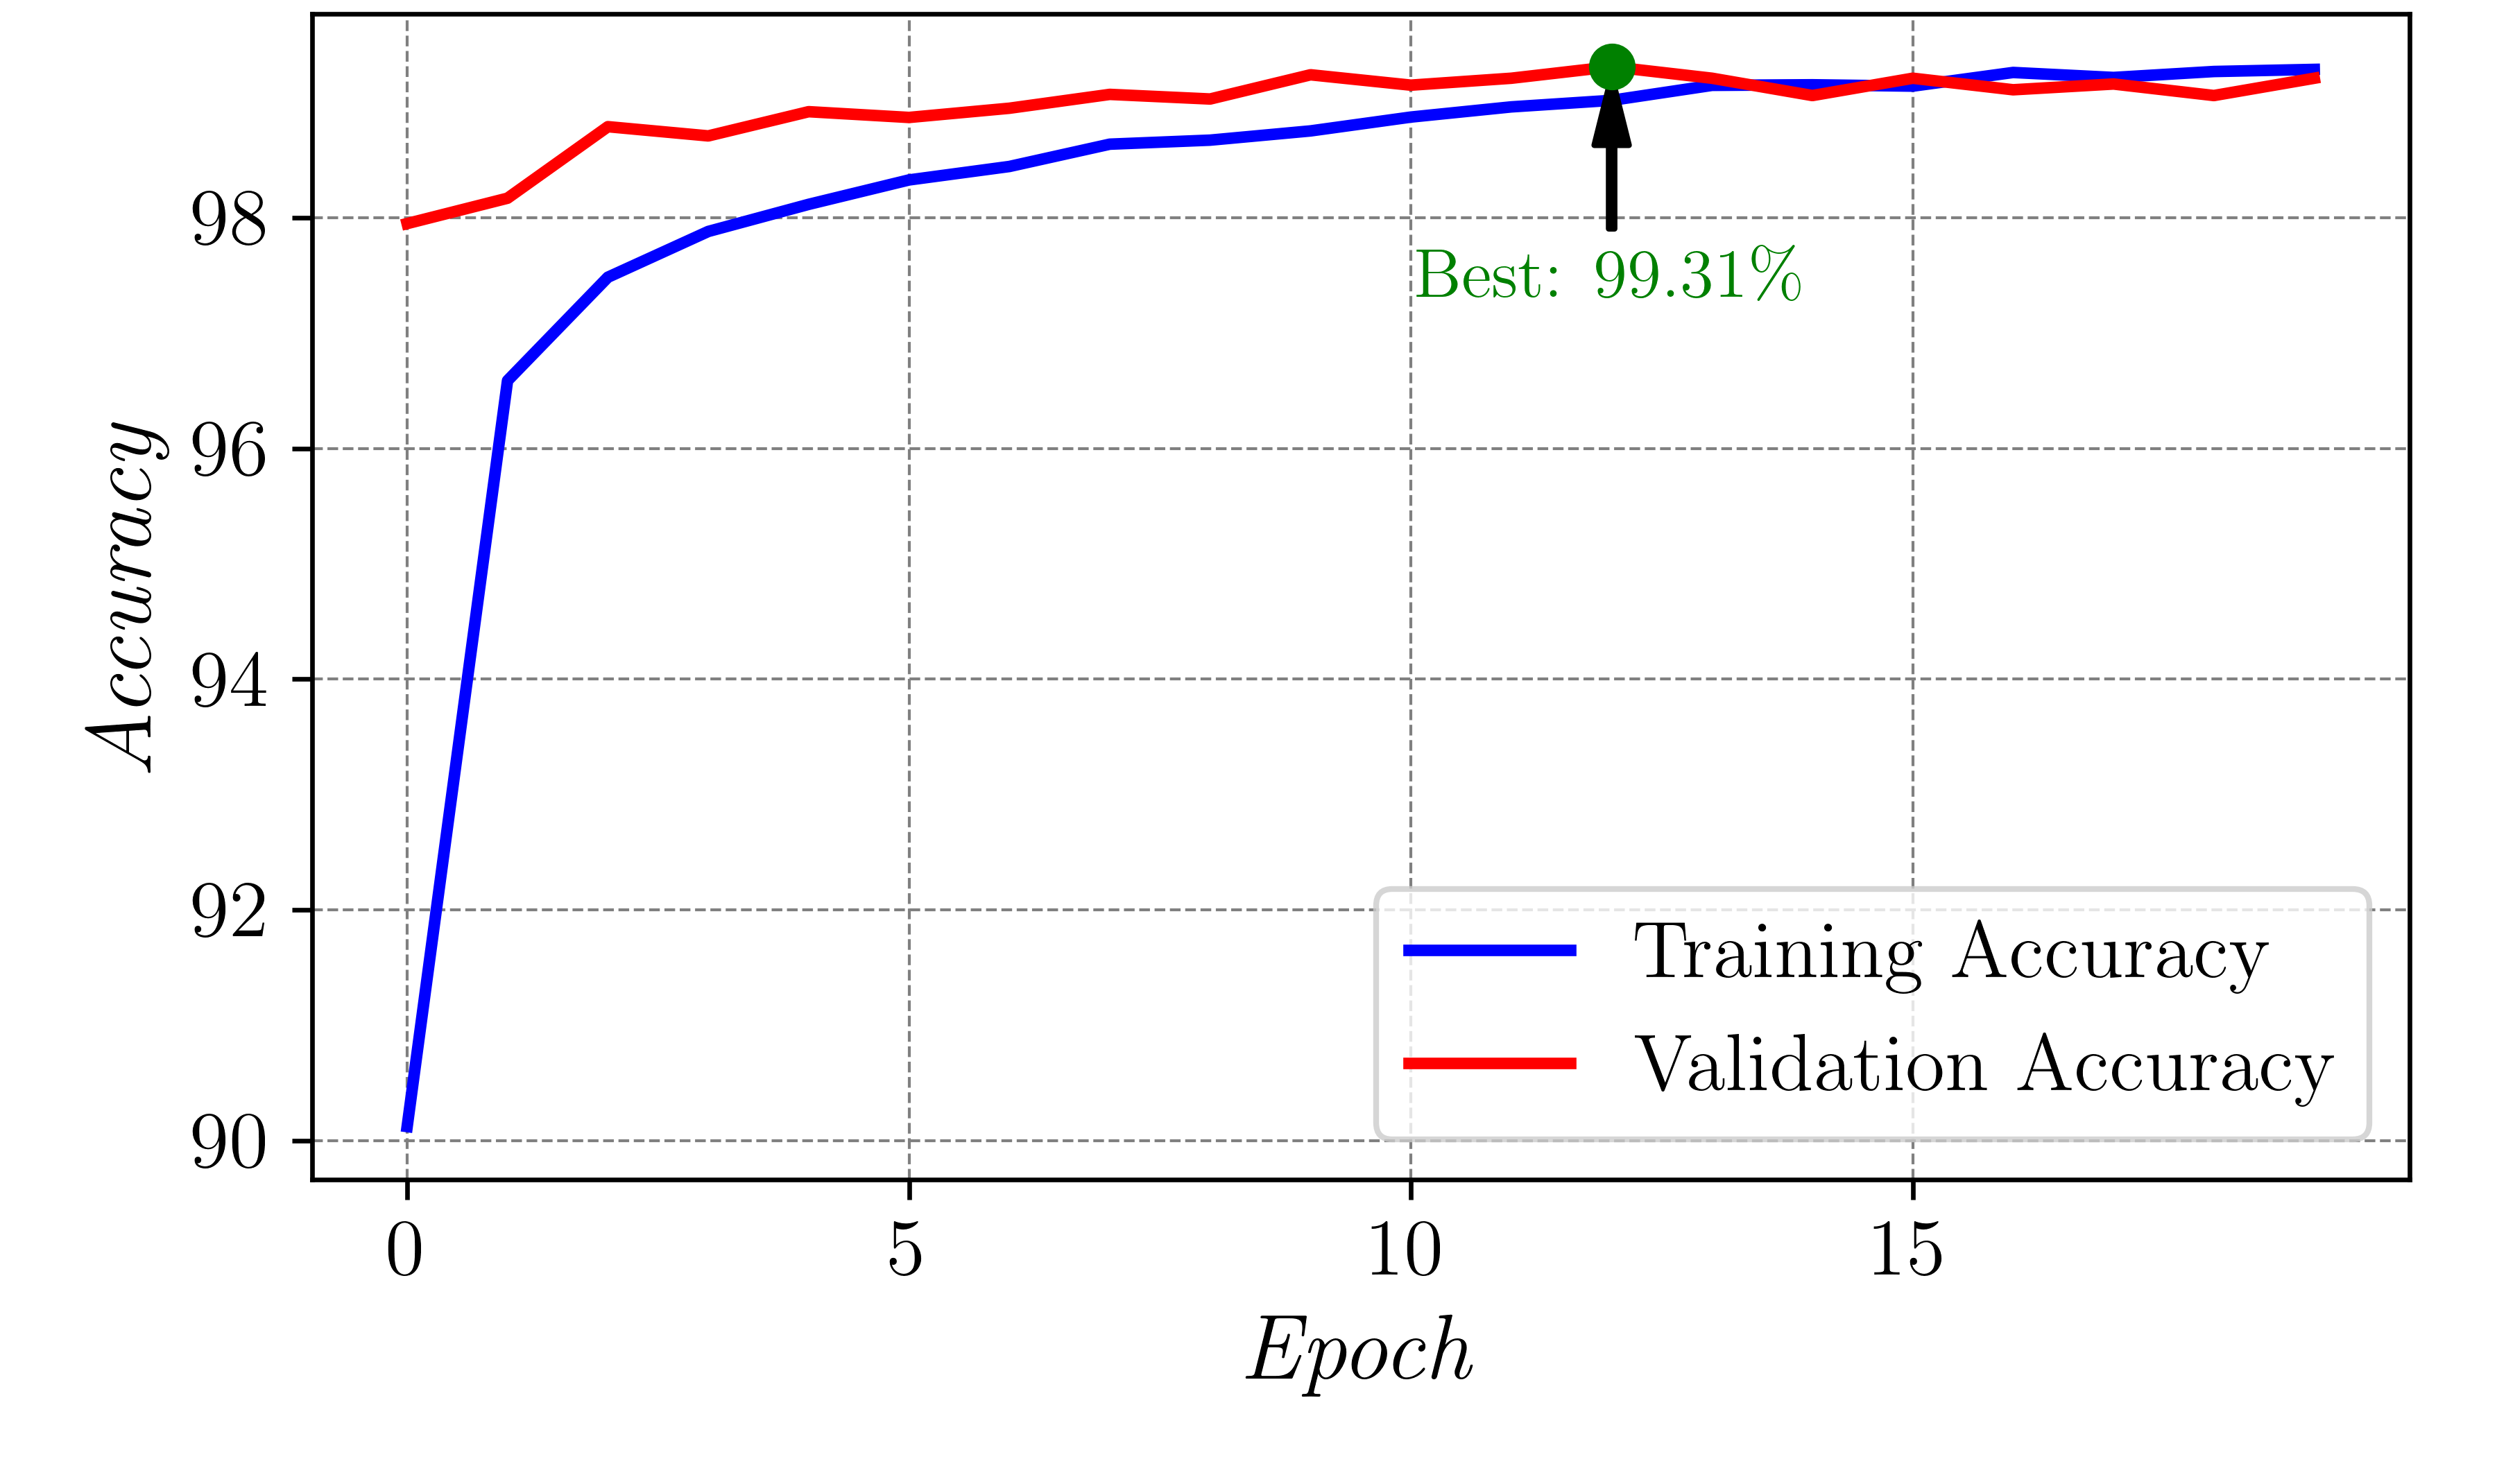
\includegraphics[width=0.7\textwidth]{img/result/accuracy_plot.png}
    \caption{Accuracy over epochs for training and validation}
    \label{f:accuracy_plot}
  \end{center}
\end{figure}

\begin{figure}
  \begin{center}
    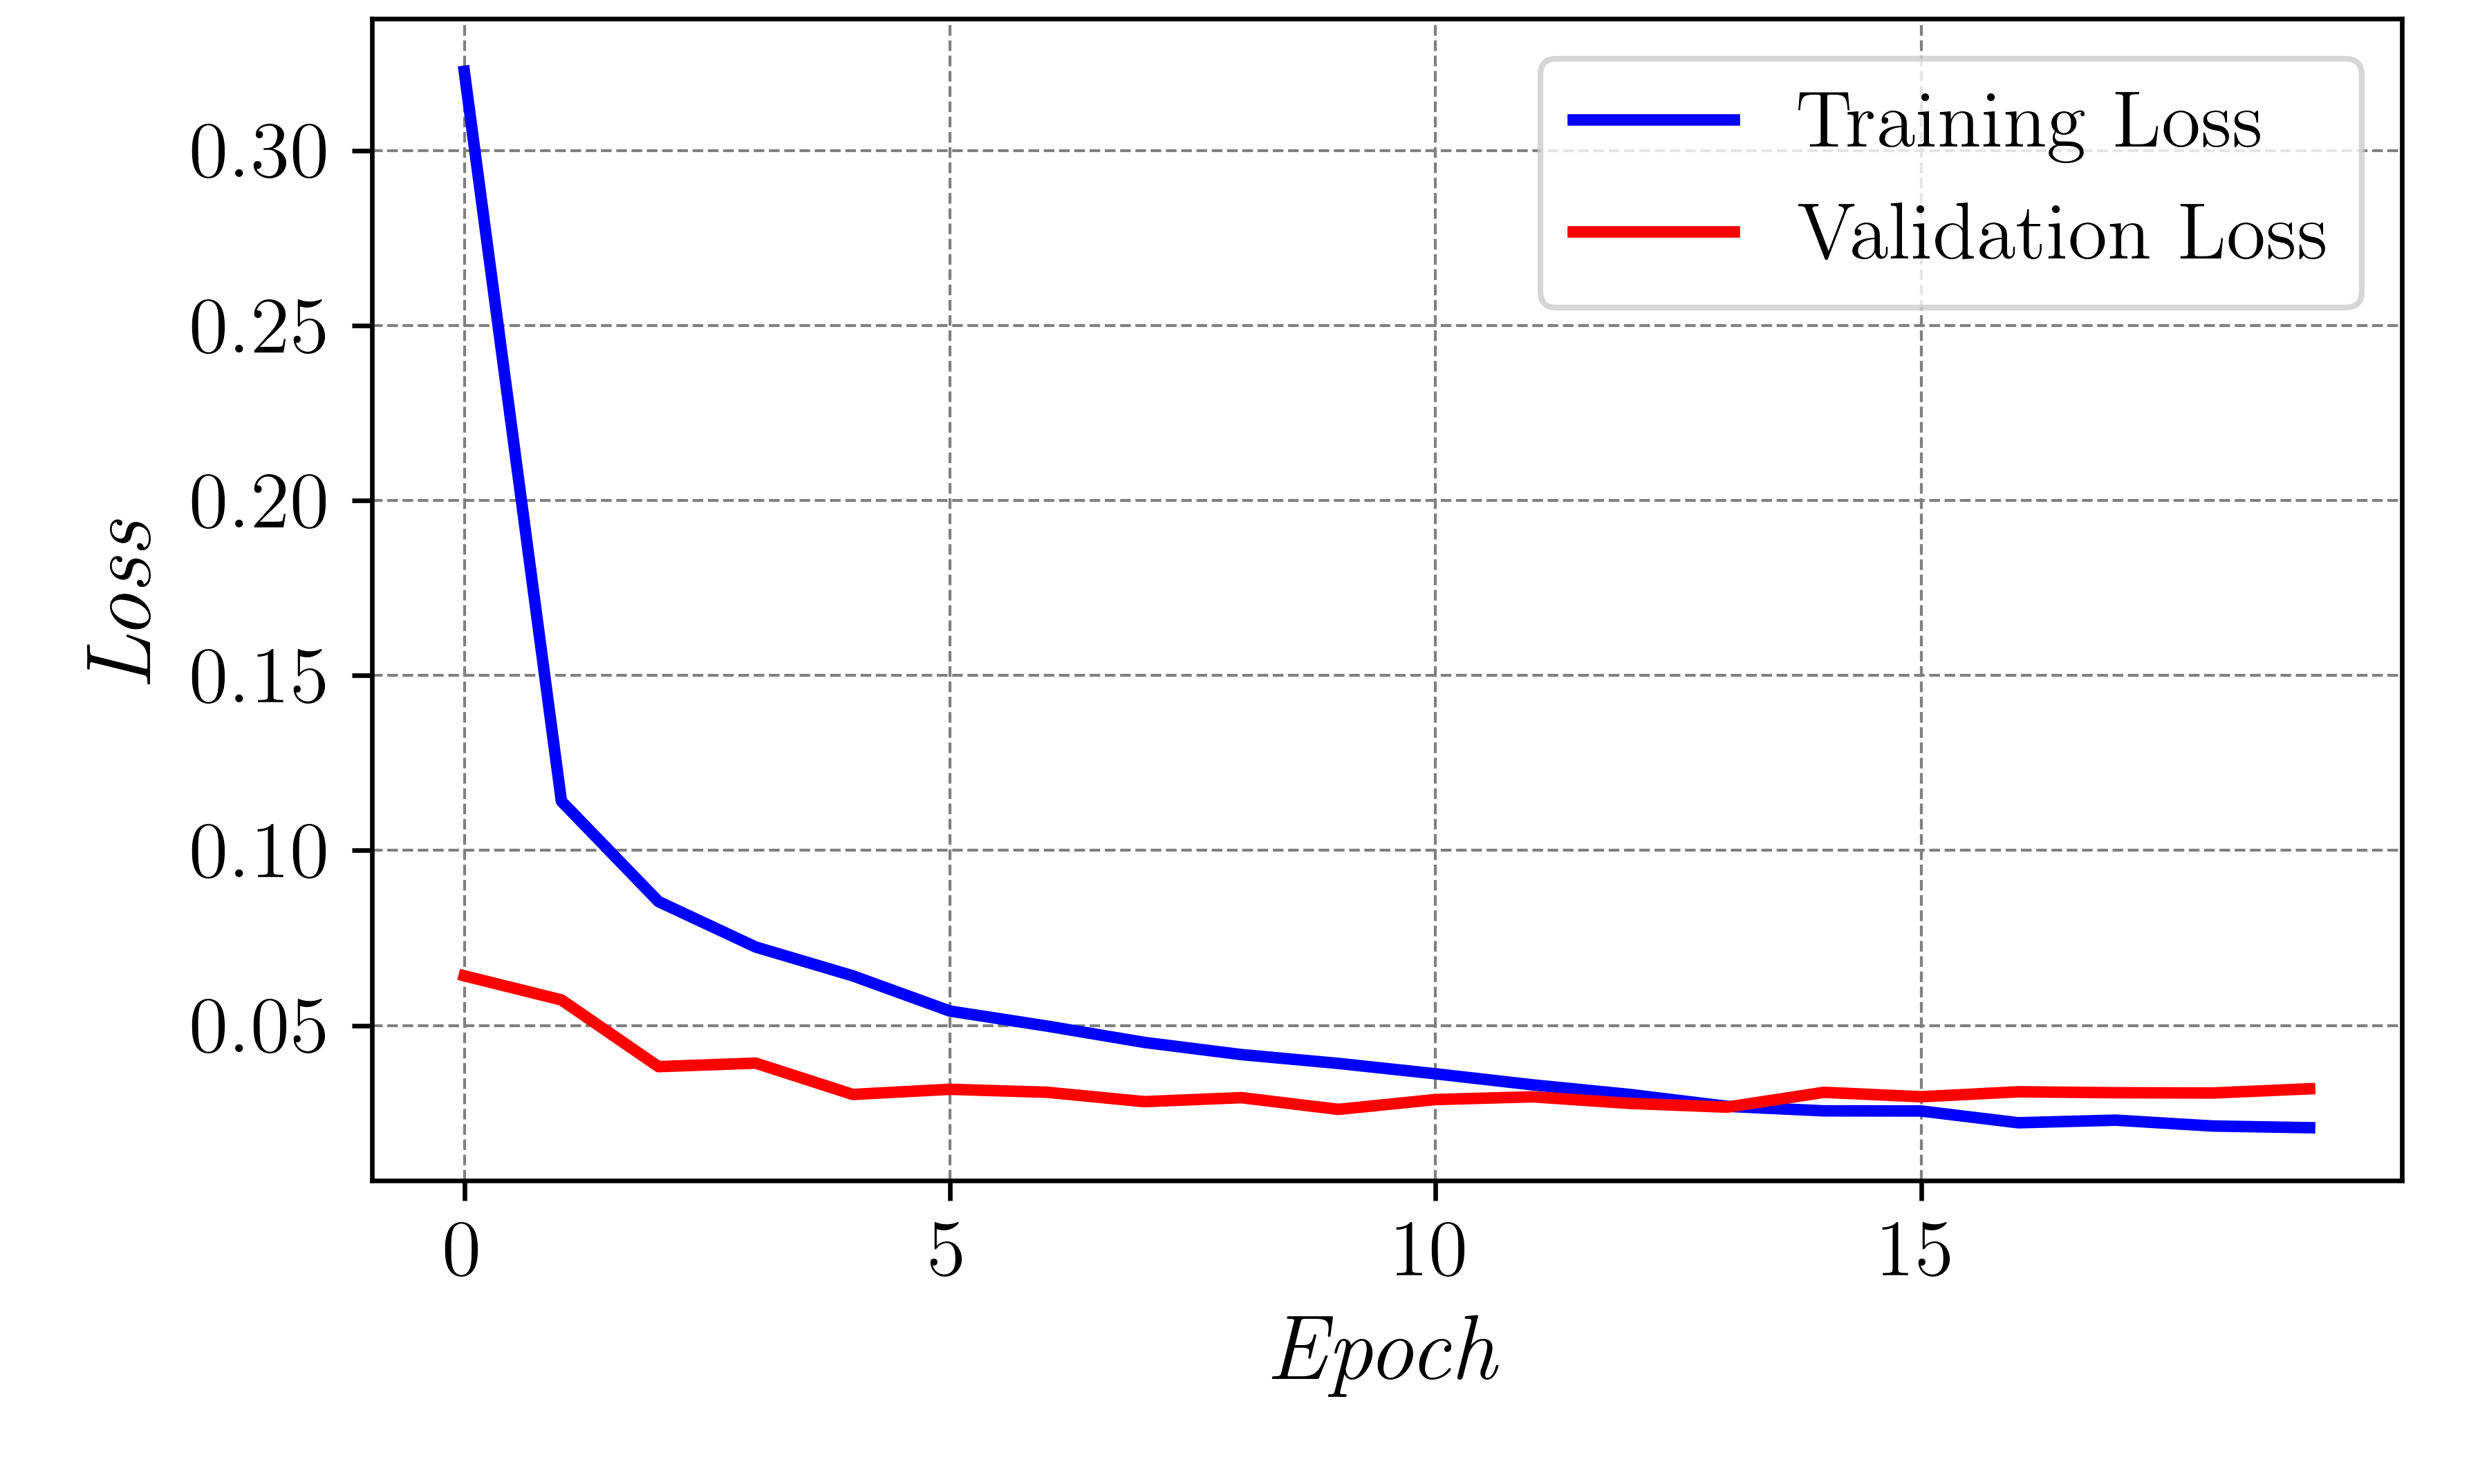
\includegraphics[width=0.7\textwidth]{img/result/loss_plot.png}
    \caption{Loss over epochs for training and validation}
    \label{f:loss_plot}
  \end{center}
\end{figure}

\begin{table}
  \centering
  \begin{tblr}{
      hlines, vlines,
      cells = {c},
      columns = {20pt},
      row{1} = {bg=lightgray!100},
      column{1} = {bg=lightgray!100,wd=48pt},
    }
    \diagbox{Pred}{True} & 0 & 1 & 2 & 3 & 4 & 5 & 6 & 7 & 8 & 9 \\
    0 & 972 & 1 & 2 & 0 & 0 & 0 & 2 & 0 & 2 & 1 \\
    1 & 0 & 1128 & 2 & 1 & 1 & 0 & 2 & 1 & 0 & 0 \\
    2 & 1 & 8 & 1013 & 3 & 0 & 0 & 0 & 5 & 2 & 0 \\
    3 & 0 & 0 & 1 & 999 & 0 & 5 & 0 & 3 & 1 & 1 \\
    4 & 0 & 0 & 0 & 0 & 973 & 0 & 2 & 2 & 1 & 4 \\
    5 & 4 & 0 & 0 & 11 & 0 & 874 & 2 & 0 & 0 & 1 \\
    6 & 3 & 2 & 0 & 0 & 2 & 7 & 941 & 0 & 3 & 0 \\
    7 & 0 & 4 & 1 & 1 & 2 & 0 & 0 & 1016 & 1 & 3 \\
    8 & 5 & 1 & 3 & 3 & 4 & 2 & 2 & 0 & 952 & 2 \\
    9 & 3 & 1 & 0 & 3 & 10 & 4 & 0 & 4 & 4 & 980 \\
  \end{tblr}
  \caption{Confusion Matrix for Model Predictions}
\end{table}

\begin{figure}
  \begin{center}
    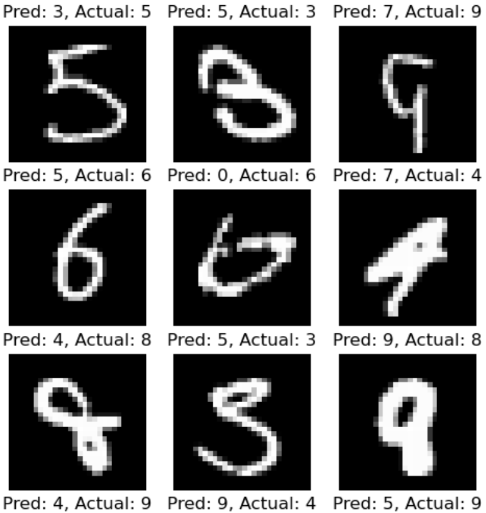
\includegraphics[width=0.4\textwidth]{img/result/wrong_samples.png}
    \caption{Examples of incorrect samples}
  \end{center}
\end{figure}
